\section{Overview}\label{overview}

\subsection{Abstract}\label{abstract}

\begin{frame}{Abstract}

\begin{itemize}
\itemsep1pt\parskip0pt\parsep0pt
\item
  Venti: A network storage system intended for archival data
\item
  A building block for a variety of storage applications

  \begin{enumerate}
  \def\labelenumi{\arabic{enumi})}
  \itemsep1pt\parskip0pt\parsep0pt
  \item
    logical backup
  \item
    physical backup
  \item
    snapshot file systems
  \end{enumerate}
\item
  A block is identified by a unique hash of it's contents
\item
  Enforce a write-once policy
\item
  Duplicate copies of a block can be coalesced
\end{itemize}

\end{frame}

\subsection{Background}\label{background}

\begin{frame}{Archival Storage}

\begin{itemize}
\itemsep1pt\parskip0pt\parsep0pt
\item
  Purpose

  \begin{itemize}
  \itemsep1pt\parskip0pt\parsep0pt
  \item
    Store data for long periods of time (forever)
  \item
    Data may not be needed frequently, but when it is needed it is often
    crucial
  \end{itemize}
\end{itemize}

\end{frame}

\begin{frame}{Prevalent Form}

\begin{itemize}
\itemsep1pt\parskip0pt\parsep0pt
\item
  Tape backup

  \begin{itemize}
  \itemsep1pt\parskip0pt\parsep0pt
  \item
    Backup data to magnetic tape
  \item
    (tar, ufsdump\ldots{})
  \item
    Full backup vs Incremental backup
  \item
    To provide backup as a central service for a number of client
    machines
  \end{itemize}
\end{itemize}

\end{frame}

\begin{frame}{Prevalent Form}

\begin{itemize}
\itemsep1pt\parskip0pt\parsep0pt
\item
  Snapshot

  \begin{itemize}
  \itemsep1pt\parskip0pt\parsep0pt
  \item
    A snapshot is a consistent read-only view of the file system at some
    point in the past.
  \item
    Each snapshot is a complete file system tree, much like a full
    backup.
  \item
    A snapshot only requires additional storage for the blocks that have
    changed, like a incremental backup.
  \item
    Always available and easy to access
  \item
    Plan 9, WAFL, AFS\ldots{}
  \end{itemize}
\end{itemize}

\end{frame}

\subsection{Venti}\label{venti}

\begin{frame}{Venti Archival Storage}

\begin{itemize}
\itemsep1pt\parskip0pt\parsep0pt
\item
  Goal: To provide a write-once archival reponsitory than can be shared
  by mutiple client machines and applications.
\item
  Block level network storage system

  \begin{itemize}
  \itemsep1pt\parskip0pt\parsep0pt
  \item
    Actually a backend storage for client apps
  \end{itemize}
\item
  Blocks addressed by hash of their contents

  \begin{itemize}
  \itemsep1pt\parskip0pt\parsep0pt
  \item
    Use SHA-1 algorithm
  \item
    Use hash value as its unique `fingerprint'
  \end{itemize}
\item
  Write-Once policy

  \begin{itemize}
  \itemsep1pt\parskip0pt\parsep0pt
  \item
    Block once written, never modified
  \item
    Modified blocks will have new address
  \end{itemize}
\end{itemize}

\end{frame}

\begin{frame}{Why SHA-1?}

\begin{itemize}
\itemsep1pt\parskip0pt\parsep0pt
\item
  SHA-1 hash function is developed by NIST
\item
  Output 160 bit hash values(20 bytes)
\item
  Probability that there will be one or more collisions:

  \begin{displaymath}
  p \leq{} \frac{n(n-1)}{2} \times{} \frac{1}{2^b}
  \end{displaymath}
\item
  Consider a large storage system contains \(10^{18}\) byte of data
  stored as 8 Kbyte blocks(\(\sim{}10^{14}\) blocks), the probability is
  less then \(10^{-20}\).
\item
  Variants of SHA-1 can produce 256, 384 and 512 bit results for future
  use.
\end{itemize}

\end{frame}

\begin{frame}{Venti Archival Storage}

\begin{itemize}
\itemsep1pt\parskip0pt\parsep0pt
\item
  Multiple clients can Share a Venti server

  \begin{itemize}
  \itemsep1pt\parskip0pt\parsep0pt
  \item
    Hash function gives an unversal namespace
  \item
    Duplication increases the utility rate of space
  \end{itemize}
\item
  Inherent integrity checking for data
\item
  Caching is simplified
\item
  Uses magnetic disk as storage technology

  \begin{itemize}
  \itemsep1pt\parskip0pt\parsep0pt
  \item
    Access time comparable to non-archival data
  \end{itemize}
\end{itemize}

\end{frame}

\section[Organization]{Data Organization}\label{data-organization}

\begin{frame}{Data Organization}

\begin{itemize}
\itemsep1pt\parskip0pt\parsep0pt
\item
  Data is divided into blocks and written to the server
\item
  Pack the fingerprints into additional blocks, called pointer blocks,
  that are also written to the server
\item
  Until a single fingerprint is obtained
\item
  Applications can use such a structure to store a single file or to
  mimic the behavior of a physical device such as a tape or a disk drive
\end{itemize}

\end{frame}

\begin{frame}{Data Organization}

\begin{figure}
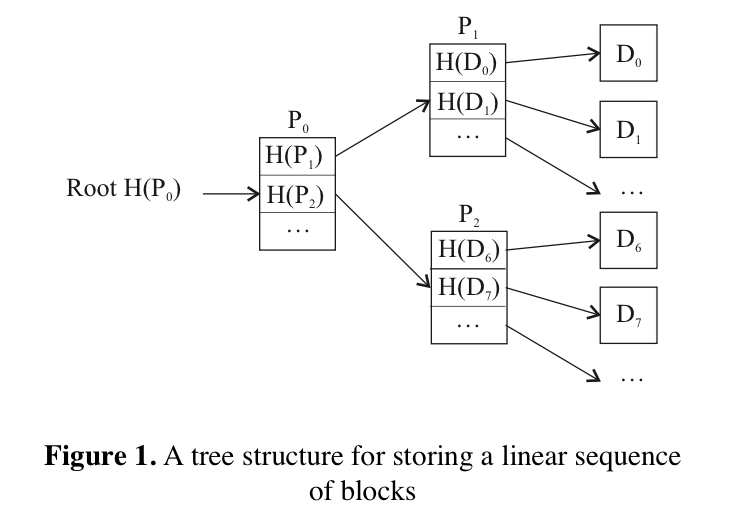
\includegraphics[width = 8cm]{pic1.png}
\end{figure}

\end{frame}

\begin{frame}{Data Organization}

\begin{itemize}
\itemsep1pt\parskip0pt\parsep0pt
\item
  Venti does not allow such a tree to be modified
\item
  But new versions of the tree can be generated efficiently by storing
  the new or modified data blocks and reusing the unchanged sections
\item
  By mixing data and fingerprints in a block, more complex data
  structures can be constructed.
\item
  For example, a structure for storing a file system may include three
  types of blocks:

  \begin{itemize}
  \itemsep1pt\parskip0pt\parsep0pt
  \item
    Directory
  \item
    Pointer
  \item
    Data.
  \end{itemize}
\end{itemize}

\end{frame}

\begin{frame}{Data Organization}

\begin{figure}
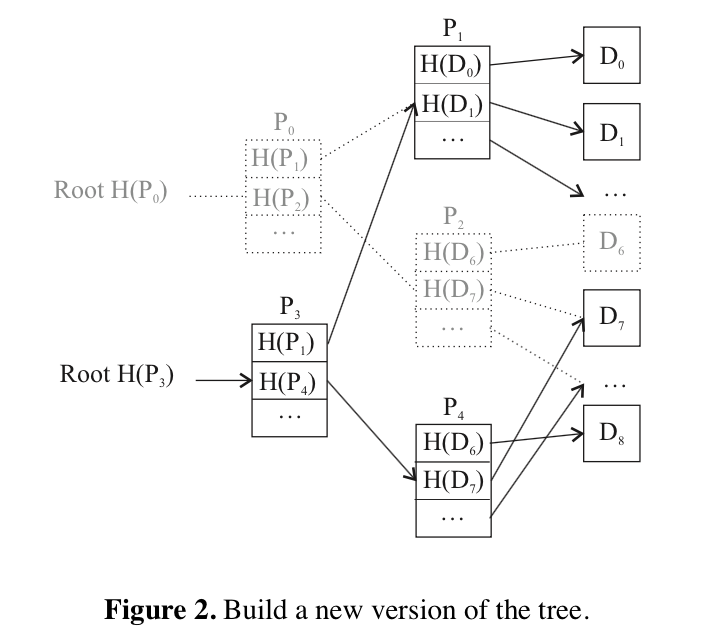
\includegraphics[width = 8cm]{pic2.png}
\end{figure}

\end{frame}

\section{Application Example}\label{application-example}

\subsection{Vac}

\begin{frame}{Vac}

\begin{itemize}
\itemsep1pt\parskip0pt\parsep0pt
\item
  Vac is an application similar to tar and zip

  \begin{itemize}
  \itemsep1pt\parskip0pt\parsep0pt
  \item
    With vac, Selected files will be stored as \newline{} a tree of
    blocks on Venti server.
  \item
    The output is always 45 bytes long,\newline{} included a 20 byte
    root fingerprint.
  \item
    `unvac' enables user to estore files from a vac archive.
  \end{itemize}
\item
  Vac writes each file as a seperated collection of Venti blocks, which
  can coalesce duplicate copies of a file
\item
  Incremental backups options can improve performance
\end{itemize}

\subsection[Phy Bak]{Physical Backup}

\end{frame}

\begin{frame}{Physical Backup}

\begin{itemize}
\itemsep1pt\parskip0pt\parsep0pt
\item
  Vac archive data at the file or logical level
\item
  Alternative approach: block-level or physical backup
\item
  Copy the raw contents of disk drives to Venti
\item
  Coalescing duplicate blocks is the main advantage
\item
  Can even mount a backup file system image from Venti
\item
  Full restore can be done in a lazy fashing
\end{itemize}

\subsection[Plan 9]{Plan 9 File System}

\end{frame}

\begin{frame}{Plan 9 File System}

\begin{itemize}
\itemsep1pt\parskip0pt\parsep0pt
\item
  When combined with a small amount of read/write storage, Venti can be
  used as the primary location for data
\item
  Plan 9 file system store snapshot on optical jukebox
\item
  magnetic disks act as a cache for the jukebox
\item
  New version of the Plan 9 file system uses Venti instead of an optical
  jukebox as its storage device
\end{itemize}

\end{frame}

\section[Implement]{Implementation}\label{implementation}

\begin{frame}{Implementation}

\begin{figure}
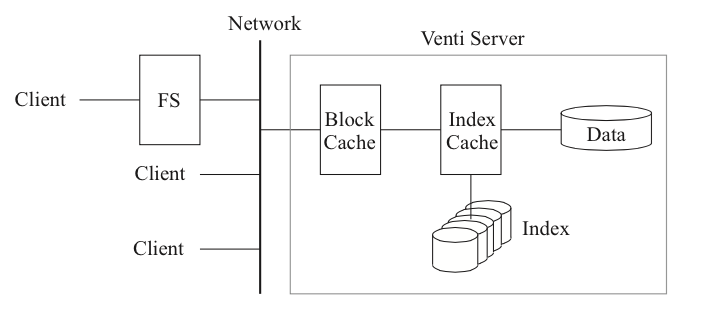
\includegraphics[width = 9cm]{pic3.png}
\end{figure}

\end{frame}

\begin{frame}{Implementation}

\begin{itemize}
\itemsep1pt\parskip0pt\parsep0pt
\item
  For data block

  \begin{itemize}
  \itemsep1pt\parskip0pt\parsep0pt
  \item
    Use Append-only log
  \item
    Blocks store on a RAID-5 array of IDE disk drives
  \end{itemize}
\item
  For Index

  \begin{itemize}
  \itemsep1pt\parskip0pt\parsep0pt
  \item
    Using a disk-resident hash table
  \item
    Index is diveided into fixed-size buckets
  \item
    Index store on 8 SCSI drives
  \end{itemize}
\item
  Additional work

  \begin{itemize}
  \itemsep1pt\parskip0pt\parsep0pt
  \item
    caching, striping, write buffering
  \end{itemize}
\end{itemize}

\end{frame}

\begin{frame}{Format of Data Log}

\begin{figure}
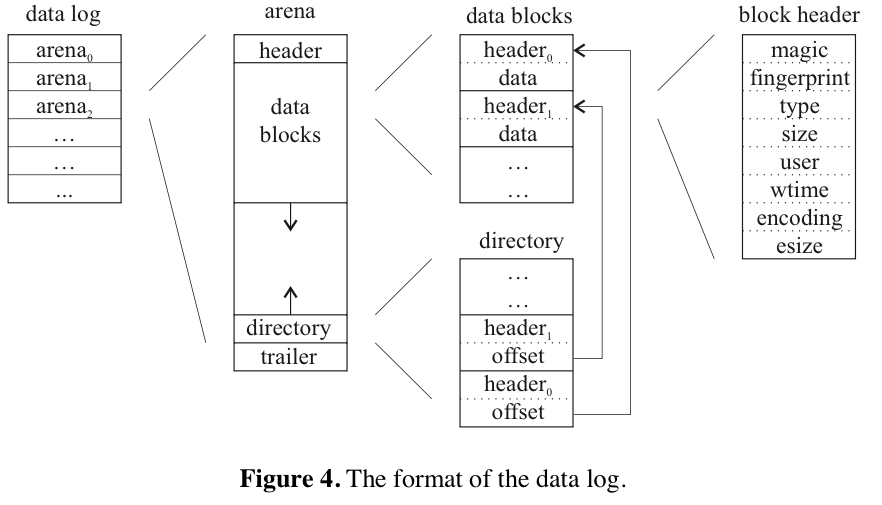
\includegraphics[width = 9cm]{pic4.png}
\end{figure}

\end{frame}

\begin{frame}{Format of Index}

\begin{figure}
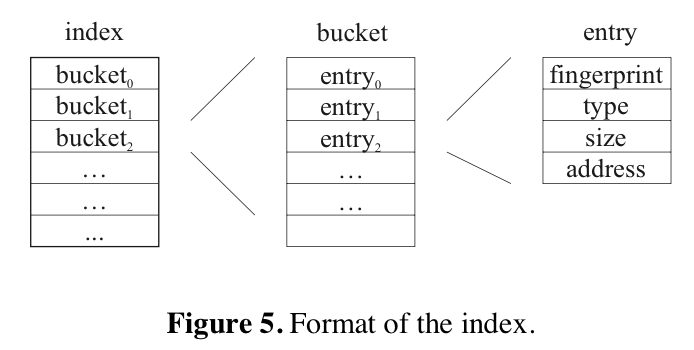
\includegraphics[width = 9cm]{pic5.png}
\end{figure}

\end{frame}

\section{Performance}\label{performance}

\begin{frame}{Performance}

The performance of read and write in Mbytes/s :

\begin{figure}

\begin{tabular}{lcccc}
\hline
           &   sequential  &  random  &  virgin  & duplicate \\
           &      reads    &  reads   &  writes  &   writes \\
\hline
uncached      &    0.9        &       0.4    &     3.7      &      5.6 \\
index cache   &    4.2        &       0.7    &      -         &    6.2 \\
block cache   &    6.8        &        -     &      -         &    6.5 \\
raw raid      &    14.8       &       1.0    &     12.4     &     12.4 \\
\hline
\end{tabular}
\end{figure}

\end{frame}

\begin{frame}{Performance}

\begin{figure}
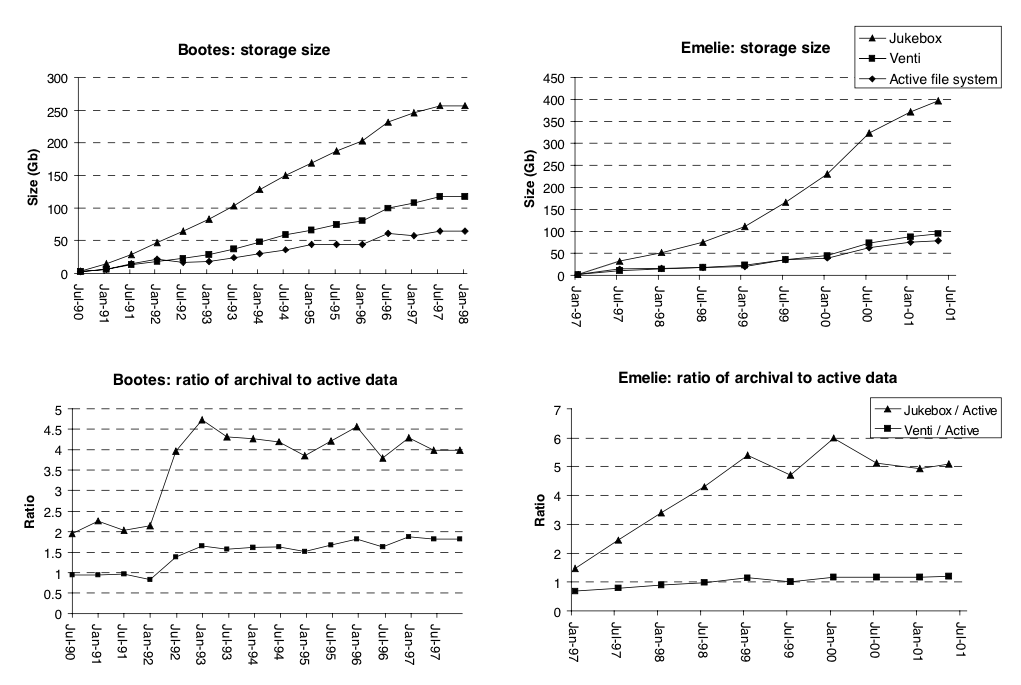
\includegraphics[width = 10cm]{pic6.png}
\end{figure}

\end{frame}

\begin{frame}{Performance}

The percentage reduction in the size of data stored on Venti :

\begin{figure}
\begin{tabular}{lcc}
\hline
&bootes &emelie \\
\hline
Elimination of duplicates & 27.8\% & 31.3\% \\
Elimination of fragments & 10.2\% & 25.4\% \\
Data Compression & 33.8\% & 54.1\% \\
Total Reduction & 59.7\% & 76.5\% \\
\hline
\end{tabular}
\end{figure}

\end{frame}

\section{Conclusion}\label{conclusion}

\begin{frame}{Conclusion}

\begin{itemize}
\itemsep1pt\parskip0pt\parsep0pt
\item
  Approach of identifying a block by SHA-1 hash is a well suited to
  archival storage
\item
  Write-once policy of a block and ability to coalesce duplicate copies
  of a block makes Venti a useful building block for many interesting
  storage application
\item
  By rapid groth in capacity of magnetic disks, it seems unlikely that
  archival data will be deleted to reclaim space

  \begin{center}
  $\Downarrow{}$\\
  Venti provides an attractive approach to archive data
  \end{center}
\end{itemize}

\end{frame}
